\documentclass{acm_proc_article-sp}
\usepackage[latin1]{inputenc}
\usepackage{amsmath}
\usepackage{amsfonts}
\usepackage{amssymb}
\usepackage{graphicx}
\usepackage{listings}
\usepackage{url}
\usepackage{havannah}
\newcommand{\black}{\texttt{Black}}
\newcommand{\white}{\texttt{White}}
\newcommand{\blacks}{\texttt{Black's}}
\newcommand{\whites}{\texttt{White's}}
\newcommand{\loc}[1]{\texttt{#1}}


\title{Learning to Bias MCTS Playouts}
\numberofauthors{2}
\author{ 
% You can go ahead and credit any number of authors here,
% e.g. one 'row of three' or two rows (consisting of one row of three
% and a second row of one, two or three).
%
% The command \alignauthor (no curly braces needed) should
% precede each author name, affiliation/snail-mail address and
% e-mail address. Additionally, tag each line of
% affiliation/address with \affaddr, and tag the
% e-mail address with \email.
%
% 1st. author
\alignauthor
James Pettit \\
       \affaddr{U.C. Santa Cruz}\\
       \affaddr{Santa Cruz, California}\\
       \email{ james.l.pettit@gmail.com }
% 2nd. author
\alignauthor
David Helmbold \\
       \affaddr{U.C. Santa Cruz}\\
       \affaddr{Santa Cruz, California}\\
       \email{dph@soe.ucsc.edu}
}

\begin{document}


\maketitle

\begin{abstract}
Monte-Carlo Tree Search (MCTS) 
grows a partial game tree and uses a large number of random simulations to
approximate the values of the nodes.   
It has proven effective in games with such as Go and Hex where the large search space and
difficulty of evaluating positions cause difficulties for standard methods.
The best MCTS players use carefully hand-crafted rules to bias the random simulations.
Obtaining good  hand-crafting rules is a very difficult process, as even rules promoting better
simulation play can result in a weaker MCTS system~\cite{gelly2006modification}.
Our Hivemind system uses evolutionary strategies to automatically learn effective rules for biasing the 
random simulations.
We have built a MCTS player using Hivemind for the game Hex. 
The Hivemind learned rules result in a 90\% win rate against a baseline MCTS system, and 
significant improvement against the computer Hex world champion, MoHex.
\end{abstract}

\section{Introduction}
Abstract strategy games provide an attractive testbed for artificial intelligence and machine learning applications. The game framework provides immediate feedback on algorithm performance. The choice of game and rules can also be experimentally varied to give a range of difficulty and computational complexity levels. Starting with mathematical game theory research, the most common technique for game AI has been brute force search of the tree of legal moves. This technique, highly tuned and optimized, is what led to Chinook's ascendance to World Champion in 1994 and Deep Blue's eventual victory in 1997 over then World Champion Gary Kasparov. These victories cemented brute force tree search as standard techniques in abstract strategy games, to the point where computers constructing endgame tables have been strong enough to find sequences lasting for hundreds of moves. Kasparov himself suggested a version of Chess that allowed the player to consult a computer for move advice. Chinook went so far as to solve checkers, proving that perfect play will end in a draw. 
Several games, such as  Checkers, Chess, and Othello, have good enough evaluation functions and few enough legal moves so that that brute force tree search techniques can be effective.

In contrast, cutting and connecting games like Go, Hex, and Havannah, have much larger search trees and long-range interactions make it difficult to create accurate evaluation functions.
In these domains, Monte-Carlo Tree Search (MCTS) has proven effective~\cite{}, 
with the world champion Go and Hex players both using MCTS~\cite{}.
MCTS picks its next move by growing a partial game tree while using
a large number of randomized simulations to evaluate the possible moves.
Each simulation first uses a child-selection policy to navigate through the partial game tree.
After reaching a leaf of the partial game tree, a randomized continuation policy is used to complete the game 
and determine a winner.  
Finally, an update policy is used to update the partial game tree with the result of the simulation.
Although all three policies have an effect on the algorithm's playing strength, here we focus on
continuation policies for the game Hex.
Section~\ref{mcts} contains a fuller description of MCTS.

MoGo specifically, and Go programs in general, have the benefit of a rich history of play. Thousands of expert games are available for analysis. Some approaches to improving the simulation policy have focused on using expert games in training weights to direct the playout~\cite{chaslot2010adding}. More generally, common patterns are used in a hand-crafted policy to select ``urgent'' moves to play in a local area around the last played move. Hex does have one simple pattern in the form of a bridge~\cite{anshelevich2002hierarchical}, but few easy paths to crafting a better continuation policies.

The Hivemind approach automatically learns better continuation policies from self-play. 
The usual process of improvement requires hand-tuned weights that bias the continuation policy. 
Any change must be tested to detect the change in strength it gives,
and different weight parameters can have synergistic effects.
Small changes in overall algorithm strength require thousands of games of testing to detect. 
Often the improvement made by a small change in weight can be so small it will go unnoticed. 
Automatic weight tuning can improve this process, but still requires thousands of games to test. 
Recent work in this area has focused on learning weights for a small number of patterns using expert knowledge and reinforcement learning~\cite{silver2009monte}. 
Hivemind is an alternative approach using evolutionary learning. 
Because it relies on self-play, Hivemind avoids the need for extensive expert knowledge or a strong outside player.
Although our experiments have focused on Hex, 
the Hivemind framework is suitable for generic Monte-Carlo Tree Search, and has been implemented for
both Go and Hex.

The continuation biases learned by Hivemind dramatically improve the playing strength of simple MCTS players.
Our experiments show that the Hivemind biases have a 90\% win rate over an unbiased continuation policy,
and about 85\% win rates over two other continuation policies that favor local moves.  
Hivemind also wins 6.5\% of its games against the world champion MoHex.
Although 6.5\% indicates that there is still a lot of room for improvement, 
we note that the other simple policies were unable to win \emph{any} games against MoHex. 
Furthermore, Hivemind is improving only the continuation policy, 
improvements in the child-selection and tree updating policies could have greatly synergistic benefits.

The evolutionary strategies approach used by Hivemind is surprisingly stable.
In 10 different evolutionary runs, the win rates over the unbiased continuation policy remained
between 87\% and 93.5\%.  
Furthermore, the learned strategies generalize well to different board sizes.
Despite using $7 \times 7$ boards for faster training, 
the learned biases performed as well (and usually better!) against the simple policies on $11 \times 11$ and $13 \times 13$ boards.

The remainder of the paper begins with some background on the game of Hex in Section~\ref{s:hex} and
an overview of MCTS in Section~\ref{mcts}.
The Hivemind system is presented in Section~\ref{hivemind}
and Section~\ref{results} describes our experimental setup and results.




\section{Background: The Game of Hex}
\label{s:hex}
Hex is a two player, full-information, abstract strategy game played on an $N$x$N$ grid of hexagons. The players are denoted by  a color, either \black{} and \white. 
The players alternate placing markers of their color on empty hexagons. 
The object of the game is to form an unbroken chain from one side of the board to the other. 
Figure \ref{fig:13x13inprogress} shows an example game in progress on a 13x13 board, note that the numbers indicate
the order in which the markers were played and have no effect on the game.
Figure \ref{fig:13x13finished} shows the final position, \black{} having just played the winning move (71), completing an unbroken chain connecting both his sides. 

Hex is a cutting and connecting game that
has properties that make it attractive for AI research. 
Once placed, a piece never leaves the board. 
The only criterion for a legal move is that the hexagon be unoccupied (empty). 
Gale '79 proved the game cannot end in a draw, simplifying minimax methods. 
Nash, one of the inventors of the game, used a strategy stealing argument to prove the existence of a winning strategy for the first player, but the proof is by reduction and offers no insight into the winning strategy.
Solutions for all opening positions for 7x7 and 8x8 boards have been found~\cite{henderson2009solving}. 
A good portion, but not all of the 9x9 openings have also been solved. 
Nash proposed 11x11 as the ideal board size, but 13x13 has been more common in competitions, especially as the ability of computer players improves.

There are three exceptionally strong Hex programs.  Gabor Melis' \emph{Six} is the previous world champion (up to 2007). 
Six uses traditional alpha-beta search with an evaluation function based on an electrical circuit model (proposed by Anshelevich 2002)~\cite{anshelevich2002hierarchical}. 
\emph{Wolve}, from the University Alberta, also uses the Anshelevich algorithm, but more aggressively prunes provably inferior moves. 
\emph{MoHex}, also from Alberta, is based on the newer Monte-Carlo Tree Search technique, leveraging the open source \emph{Fuego} library. 
MoHex is the current world-champion, having finished ahead of Wolve in 2008, 2009 and 2010.

Go is a much older game than Hex or Havannah, and much research has been done on Go playing algorithms. 
Despite its simpler rules, Hex has a similar branching factor and position evaluation complexity as Go. 
Although we emphasize Hex here, the techniques discussed generalize to any large branching game played on a regular board
(such as Go or Havannah).

\begin{figure}[tb]
\resizebox{3.5in}{!}{	\begin{HexBoard}[board size=13]
		\HGame{c4,f6,e11,i8,h8,i1,i6,d5,i3,h9,h5,h4,i4,g9,f9,g8,f7,f8,e8}
	\end{HexBoard}
	}
	\caption{13x13 Hex Game, \white{} to play.}
	\label{fig:13x13inprogress}
\end{figure}

\begin{figure}[tb]
\resizebox{3.5in}{!}{	\begin{HexBoard}[board size=13]
		\HGame{c4,f6,e11,i8,h8,i1,i6,d5,i3,
				   h9,h5,h4,i4,g9,f9,g8,f7,f8,
				   e8,e9,c10,k8,c9,g6,g7,c11,
				   d10,h6,h7,i5,j5,j4,k4,k3,
				   m2,l3,m3,l4,c6,e11,l5,m4,
				   d11,b7,e6,d12,c12,c7,e7,f5,
				   e5,d9,d8,f4,e4,f3,a2,e3,d6,
				   c3,d3,d4,b5,e2,d2,d1,e1,b13,
				   c13,c5,b6}
	\end{HexBoard}
	}
	\caption{Finished 13x13 Hex Game, \black{}'s play 71 (at \loc{b6}) gives him an unbroken path from top to bottom.}
	\label{fig:13x13finished}
\end{figure}


\section{Monte Carlo Tree Search} \label{mcts}

\begin{figure}
	\begin{center}
%	\centerline{\begin{HexBoard}[board size=5]
%		\HGame{a3,c2}
%	\end{HexBoard}
%	}
	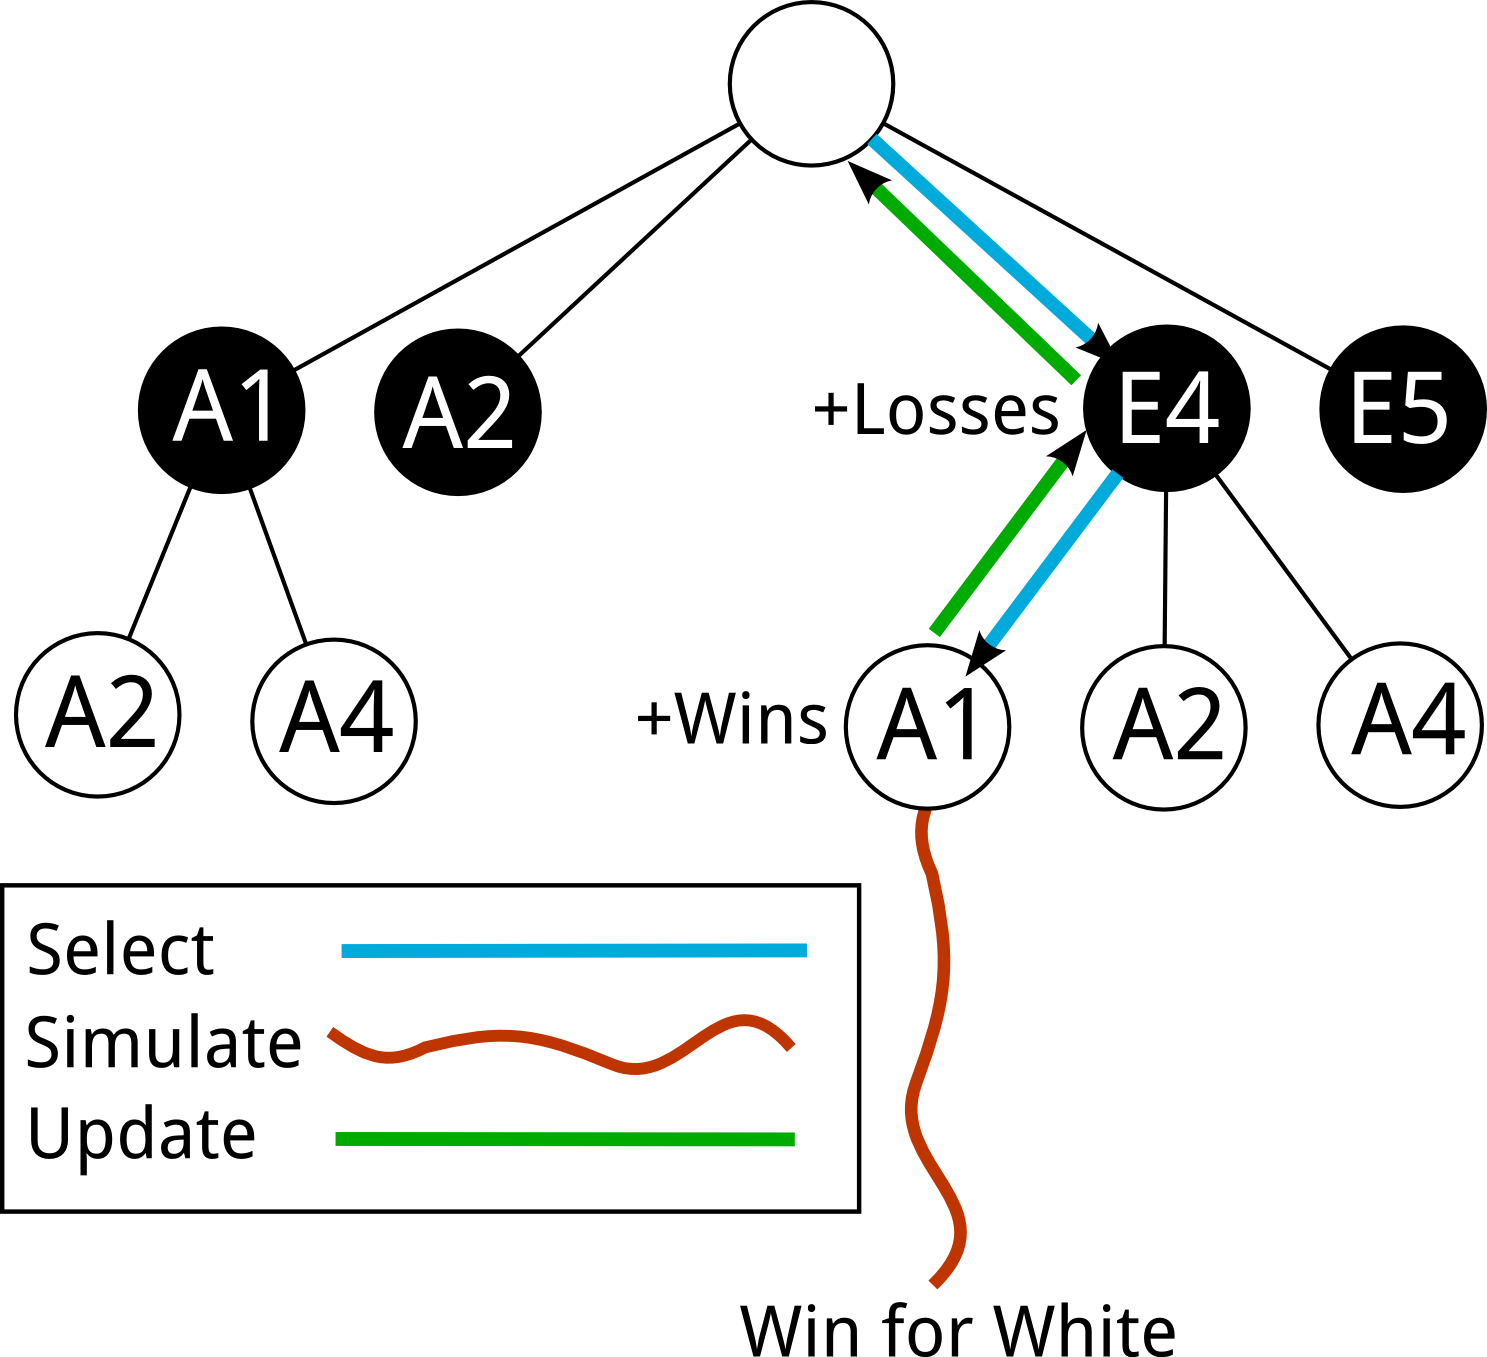
\includegraphics[width=3.0in]{graphics/tree.png}
	\end{center}
	\caption{Partial MC Search Tree}
	\label{fig:tree}
\end{figure}

%As stated, the current top computer Hex player, MoHex, uses the open-source Fuego implementation of Monte-Carlo Tree Search (MCTS)~\cite{mohex}. 

The basic Monte-Carlo technique for Computer Go was proposed by Bru\"{u}gmann~\cite{brugmann1993monte}. His program \emph{Mango} effectively used a ``flat'' search tree (1-ply) and simply ran simulations from each candidate move to estimate its value. To contrast, MCTS uses Monte-Carlo simulations to grow a partial  search tree. 
The UCT algorithm was developed alongside MCTS to direct the growth of the search tree~\cite{gelly2006exploration}. 
At any point, the search can be stopped and the current state of the tree used to select a move to play. 

All nodes in the tree correspond to a fixed board position, i.e. the occupancy state of the board and which player is next to move. 
Nodes also have statistics associated with their position:  the number of winning simulations performed that used the node, and the total number of simulations that included the node. 
For each simulation the algorithm will start at the root node, recursively traverse the (partial) tree until it reaches a leaf node.
The simulation continues from the position represented by this leaf node until a winner is determined.
The result of the simulation used to update the statistics at nodes in the tree.
If the leaf node has been visited enough times (50 in our case), then it is expanded and nodes for all possible moves from 
that position are added to the search tree.

The effectiveness of MCTS depends on three policies:
\begin{itemize}
\item{The \emph{child-selection} policy recursively traverses the tree, selecting promising moves for further exploration.}
\item{The \emph{continuation} policy randomly or semi-randomly ``plays out'' the game from a leaf position in the tree until a final position.}
\item{The \emph{update} policy modifies the win/loss statistics of nodes based on the simulation results, and determines when to grow the search tree.}
\end{itemize}
Figure \ref{fig:tree} shows a partial Monte-Carlo search tree for the given position. In the example, the child-selection policy visited the node for \texttt{Black E4}, then \texttt{White A1}. 
The continuation policy ran, completing the game from the positiion with \texttt{E4} occupied by \black\ and \texttt{A1} occupied by \white.
This resulted in a loss for \black. 
The update policy choose to update all nodes along the visited path, incrementing the wins for \white\ moves and incrementing the losses for \black\ moves.

\begin{lstlisting}[float,frame=single,language=Python,caption=MCTS Algorithm Pseudocode]
def search(root):
  for i in range(simulations):
    step(root)

def play_from(node) returns outcome:
  if node.visits < threshold:
    outcome = simulate(node)
  else:
    child = select(node)
    outcome = play_from(child)
  if outcome is win for node.player:
    node.wins++
  node.visits++
  return outcome
\end{lstlisting}

\subsection{Child Selection Policy}
The \texttt{select} function defines the child selection policy. It must return the child of the given node to step into next. 
In general, child selection must trade off between \emph{exploitation} and \emph{exploration}. 
It is important to ``exploit" those child nodes with high win-rates, both
to discover possible weaknesses that would result in the opponent winning and to obtain accurate win-rate estimates. 
Simultaneously, a child with a low number of visits must also be explored since a low win-rate
could be due to a few unlucky simulations.
This exploration/exploitation tradeoff is related to a variance reduction problem.  
We want very low variance on the estimates for the good moves in order to maximize the chances of making the best move.
On the other hand, if the variance of a seemingly poor move is very high, then there is a significant chance that that move
could actually be very good.

One way to balance this exploration/exploitation trade-off is the Upper-Confidence for Trees algorithm (UCT). 
UCT incorporates the win-rate of a child with a term that increases in value as the ratio of the child's visits to its parents decreases. 
Eventually, no matter how bad the estimated value of a position is, it will be re-visited and the estimate updated. 
UCT has several variations, but the ``pure'' version has been proven to eventually yield the correct minimax value of a position, given an infinite number of simulations~\cite{gelly2006exploration}.

The UCT priority of a child node is:
\[
	\texttt{child.winrate} + C*\sqrt{\frac{\log{(\texttt{parent.visits})}}{\texttt{child.visits}}}.
\]

The \emph{exploration coefficient}, $C$, can be varied to increase or decrease the level of exploration versus exploitation. Note that a very low value will yield a function that relies almost exclusively on the estimated win-rate of a position, while a high value will visit nodes more equally, placing less emphasis on the estimated value.

\subsection{Continuation Policy}

The \texttt{continuation} function plays out the rest of the game from the current position. 
The simplest policy, which we call the \emph{default policy},
 plays uniformly at random from the legal moves until the game ends (in Hex, when one player has a winning path). 
The continuation policy has a large effect on the strength of the MCTS player.
% and the Go literature has a large body of work dedicated to improving it.
Initial research in MCTS Go players focused on using a strong continuation policy, with expert-derived heuristics to select the next move~\cite{chaslot2010adding}. 
The top Computer Go programs all have complex hand-crafted policies with rules to examine the current position and select a ``good'' move to play, possibly with a stochastic choice between several candidates. 
Only when none of the rules match do they fall back to a uniform random move. 
It was quickly found that building a stronger continuation policy does not guarantee better performance when used in the full tree search~\cite{gelly2006modification}. 
In other words, when the continuation policies are used as players, the relative strengths of the continuation policies are poor predictors
of how well the MCTS algorithms relying on these continuation policies will perform.
This surprising result may be due to stronger continuation policies under-exploring the search space.
In any case, this means that hand crafting an effective continuation policy requires benchmarking and frequent tests of the entire
MCTS system as small changes to the simulation policy can have unpredictable effects on overall performance.
This illustrates the need for automated systems for tuning the continuation policy.

Another constraint on the continuation policy is its speed.  
MCTS algorithms require large numbers of random simulations to compute accurate statistics and select good moves, therefore the continuation policy must be not be overly complex and implemented efficiently.

\subsection{Update Policy}
Once a simulation is finished, the result is used to update the search tree.
Basic MCTS systems updated the win and visit statistics only along the traversed path.
It was quickly discovered that more aggressive update strategies are often profitable.
One simple example of this is the All-Moves-As-First (AMAF) heuristic~\cite{}
that exploits the fact that moves played in a simulation could have been played in any order. 
Thus, a move deep in the simulation could be fictitiously treated as the ``first'' move from an intermediate position. 
In addition to updating the statistics of the nodes in the path, all children of nodes on the path corresponding to moves made later
in the simulation have their AMAF win and visit counts updated. 
Variations on AMAF have been tested, including Permutations AMAF, which updates a node if any permutation of the simulation contained the node's position, and Some-Moves-As-First, which attempts to restrict the number of siblings updated.

Several methods can be used to blend the AMAF results with the ``pure'' results, such as a weighted average.
Other blending functions include Cutoff and Rapid Action Value Estimation (RAVE)~\cite{chaslot2008progressive}. 
Helmbold and Parker-Wood (2009) have a summary of the various update policies and blending methods, along with experimental results showing marked improvement over the baseline of pure UCT~\cite{helmbold2009all}. 
One noteworthy conjecture is that there is no ``silver bullet'' update policy. If the simulation policy is random and unbiased, the AMAF updates might be similarly unbiased. However, a simulation policy that preferentially plays certain moves might have an unpredictable effect on which nodes receive AMAF updates. This can then propagate to which nodes are selected during the UCT selection, and have chaotic effects on the search as a whole. 

Our Hivemind experiments use only the basic update policy, updating win and visit counts for only those nodes on the traversed path.

% TODO
\textbf{does MoHex do something fancier?}
% MoHex uses one local pattern - bridge preservation, and AMAF updates with RAVE (http://webdocs.cs.ualberta.ca/~hayward/hex/#mohex)

The tree update policy also determines how the partial search tree is grown.
Generally, systems will add the possible children of a leaf to the tree after the leaf has been visited a sufficient number of times.
This number is a parameter in Hivemind, and our experiments have set it to the (untuned) value of 50.


\subsection{Biasing the Continuation -- Incorporate into earlier subsections}\label{bias}

Gelly and others have shown that using heuristics in both the expansion and playout policy can prove extremely beneficial~\cite{gelly2006modification,gelly2008achieving}. However, this can require expert knowledge (heuristics) that is hard to obtain or not available for some games (particularly new games). They also found found that improving the performance of playout policy did not guarantee an improvement in the tree search. For example, the playout policy can implicitly prune good moves, never allowing them to be played. In Go, the policy must correctly handle complicated situations like nakade (life and death). If it fails to correctly play out a complex position, the tree might fail to see an opponent response. Much time and energy has been spent on hand-tuning the policies of the top engines to correctly handle complicated tactical situations. If there is some small probability of playing a purely random move, the convergence properties of the UCT algorithm will still hold, but can require a prohibitive number of simulations.
In fact, one of the top Go engines, MoGo, uses a near-zero exploration coefficient in its child selection policy~\cite{gelly2007combining}. This puts most of the control of the search in the hands of the simulation policy.
%
%\section{Problem Statement  -- delete? Incorporate points into MCTS section?}\label{problem}
%MoGo specifically, and Go programs in general, have the benefit of a rich history of play. Thousands of expert games are available for analysis. Some approaches to improving the simulation policy have focused on using expert games in training weights to direct the playout~\cite{chaslot2010adding}. More generally, common patterns are used in a hand-crafted policy to select ``urgent'' moves to play in a local area around the last played move. Hex does have one simple pattern in the form of a bridge~\cite{anshelevich2002hierarchical}, but few easy paths to crafting a better simulation policy.
%
%It would be ideal to automatically learn a better playout policy from self-play. The usual process of improvement requires hand-tuned weights that modify the playout policy. Any change must be tested to detect the change in strength it gives. Problematically, small changes in overall algorithm strength require thousands of games of testing to detect. Many times the improvement made by a small change in weight can be so small it will go unnoticed. Automatic weight tuning can improve this process, but still requires thousands of games to test. Recent work in this area has focused on learning weights for a small number of patterns using expert knowledge and reinforcement learning~\cite{silver2009monte}. This thesis presents a slightly different approach using evolutionary learning. It solves the problem of requiring a strong outside player or expert knowledge by purely using games of self-play.
%

\section{The Hivemind System}\label{hivemind}

Hivemind is a system that learns to play abstract strategy games on a regular board. 
The system consists of three modules: the evolutionary learning process, a Monte-Carlo based UCT search tree implementation, and a ``Game Tracker interface'' used by the tree search to maintain game state information. 
The design was influenced by Fuego, although Hivemind is written in a different language (Google's Go~\cite{golang}). 
In particular, the tracker interface is very similar to Fuego's subclassing system for implementing multiple games~\cite{Fuego}. 
Hivemind's tracker interface is currently implemented for the games of Hex, Go, and Tic-Tac-Toe. 
The major contribution of Hivemind is the integration of evolutionary learning to automatically learn appropriate continuation policies.
Hivemind is also open-source software, available at \url{http://github.com/etherealmachine/hivemind}.
Preliminary work tried learning with particle swarm optimization, but we found that evolutionary strategies gave
superior results.

Using evolutionary strategies to learn continuation policies requires that the continuation policies are encoded as vectors.
We first describe this encoding.  Section~\ref{s:tracker} describes the Game Tracker module, and Section~\ref{s:es} describes the
use of Evolutionary Strategies.

\subsection{Continuation Policies and Local Patterns}
\label{s:policies}

Hivemind uses local patterns around the previous move to bias the random continuations.
Responding to an opponent's threat is often necessary in cutting and connecting games
and local patterns around the last move can be efficiently evaluated, allowing for efficient simulation.
Strong MCTS Go programs like MoGo~\cite{gelly2006modification} use hand-crafted local patterns to direct their  continuation policies.

Each empty location around this last move is a candidate local response, and a pattern database gives each of these candidates a
weight indicating its relative importance.
During a continuation play-out, a candidate local response is selected with probability proportional to its weight.
Figures \ref{fig:localpattern} and \ref{fig:encoding} show graphically how a local patterns can be mapped to an integer. 
The orange marker denotes the last move played. 
In Hex there are less than $2 * 4^6=2^{13}$ possible local patterns, and 
assigning a weight to each of these patterns creates a continuation strategy.
Thus the continuation strategies we consider correspond to an array of $2^{13}$ weights, one for each local pattern.
% TODO
\textbf{How about tenuki weights? does hivemind consider them?}
% Early experiments with tenuki weights were less successful. The default policy is only used if no legal moves exist in the local area.

In the example shown in figure \ref{fig:localpattern}, the sum of the three weights is 11. Thus, vertex A will be selected with probability $P(A) = \frac{6}{11} \approx 0.54$. 
B will be selected with $P(B) \approx 0.27$ and C with $P(C) \approx 0.18$. 
Note that $P(A)+P(B)+P(C) = 1$ so one of A, B, or C will be selected. 

\begin{figure}
	\begin{center}
	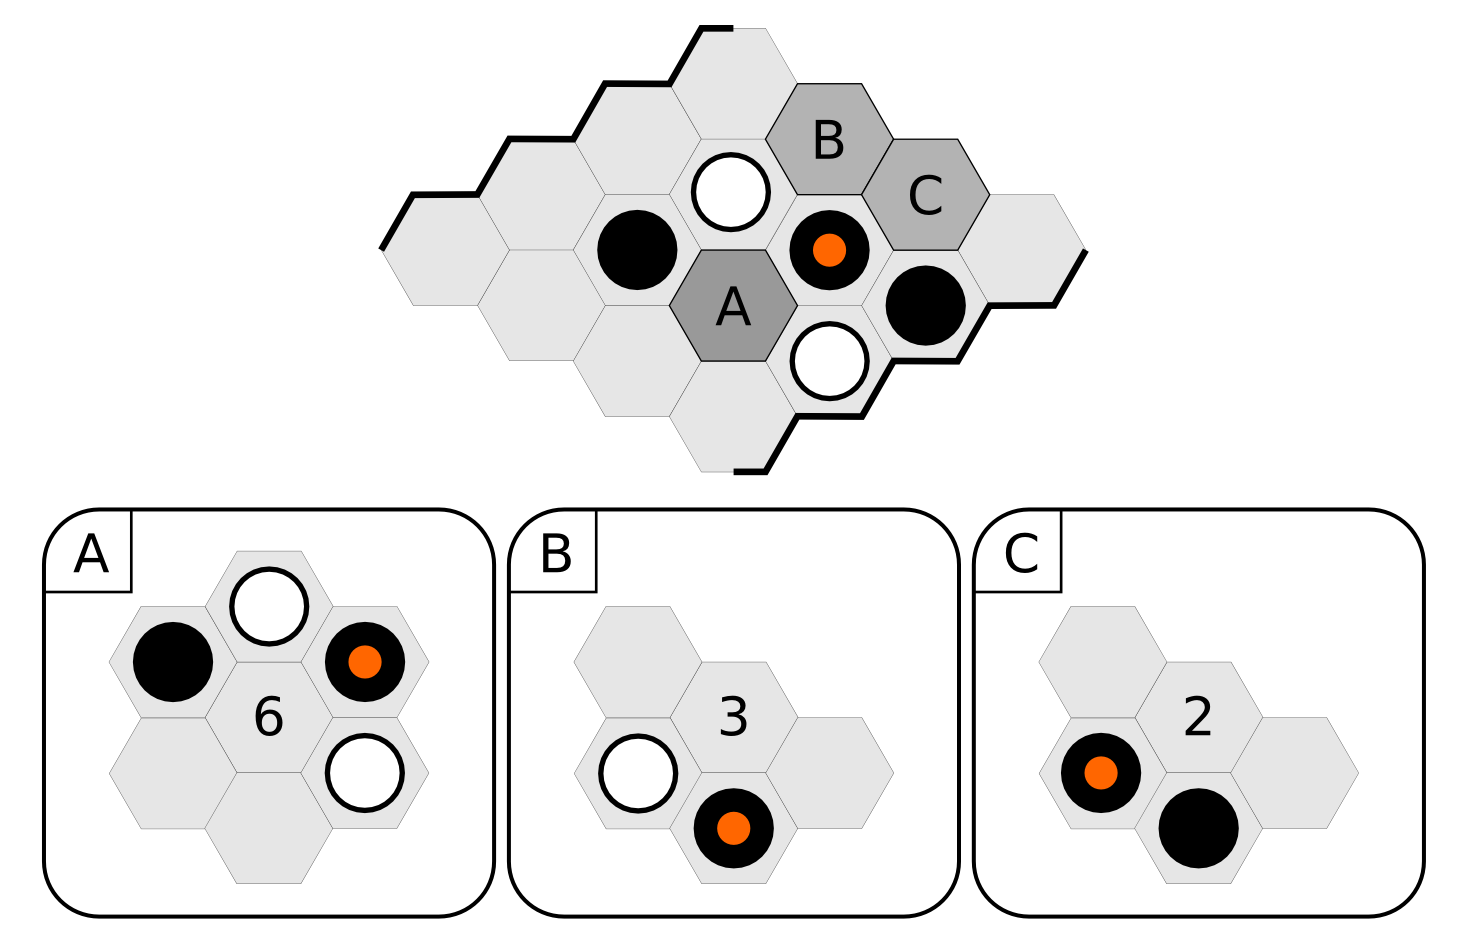
\includegraphics[width=3.0in]{graphics/local-pattern.png}
	\caption{A 4x4 board with the 3 patterns shown around \blacks\ last move. Example weights are shown in the center vertex.}
	\label{fig:localpattern}
	\end{center}
\end{figure}

\begin{figure}
	\begin{center}
	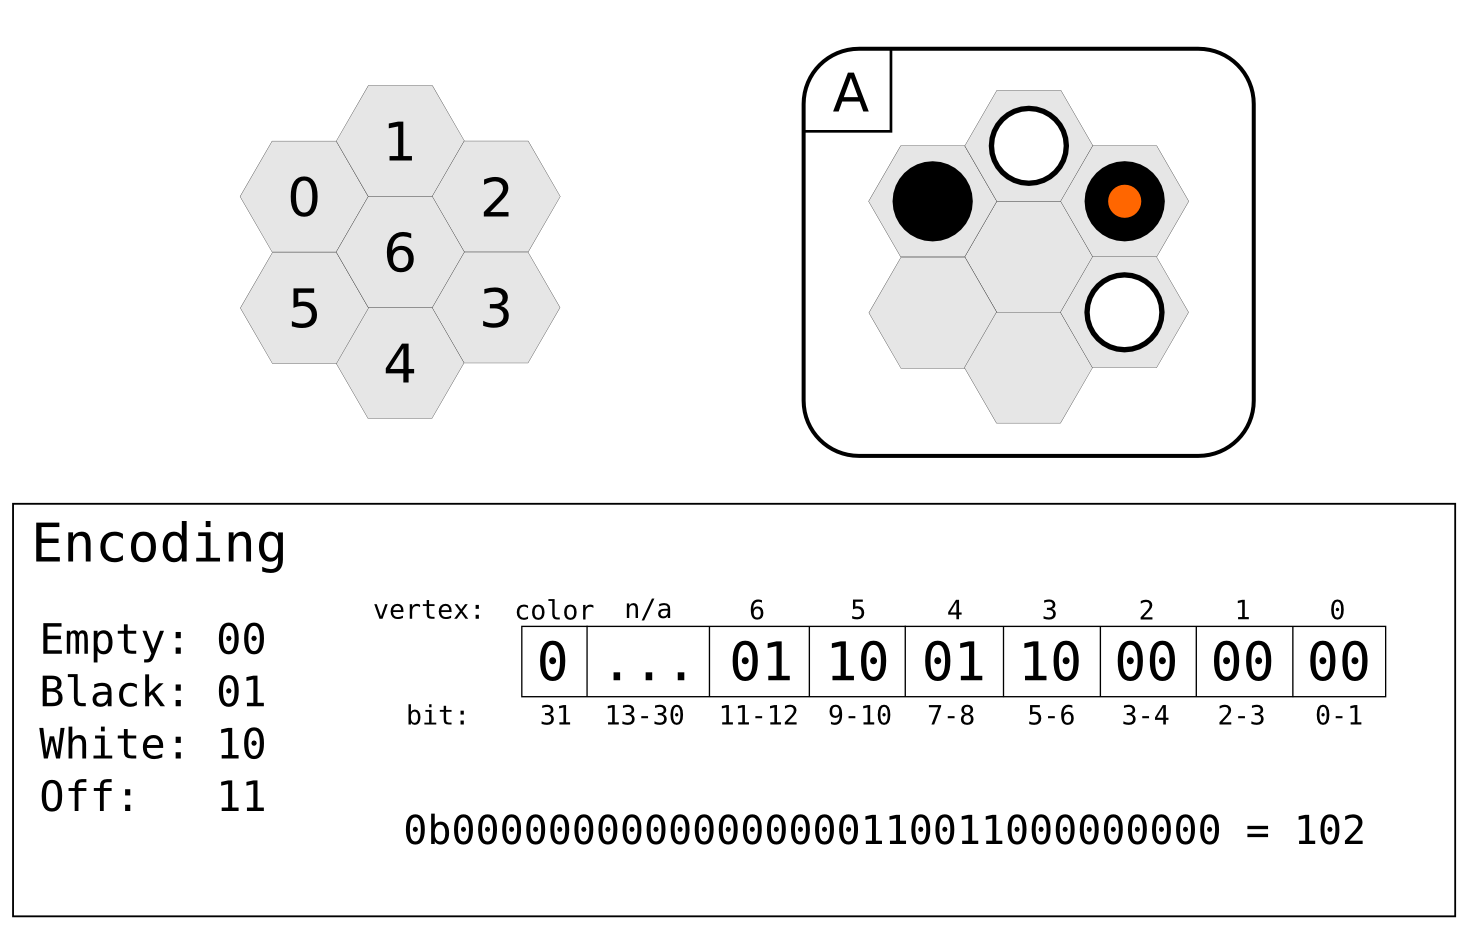
\includegraphics[width=3.0in]{graphics/weight-pattern-map.png}
	\caption{The encoding from pattern A to a 32-bit integer. Using the weight from figure \ref{fig:localpattern}, the real value 6 would be stored at position 102 in the weight map.}
	\label{fig:encoding}
	\end{center}
\end{figure}

A local pattern can assign a candidate move a weight of 0. If so, it will never be selected using the local response policy. 
If all patterns adjacent to the last move have weight 0, or if all adjacent vertices are already occupied, 
the continuation policy makes a move at random from all legal possibilities.

Although conceptually an array with $2^{13}$ entries, Hivemind implements continuation strategies as
32-bit hashmaps.  
The additional overhead is modest and the larger hashmaps  have space for additional properties (such as distance to a side).
Note that in Figure~\ref{fig:encoding} the encoding includes a color bit in the 31st position. This denotes the color to play (either \black\ (1) or \white\ (0)). 
This bit is important because \black\ and \white\ have different goals -- they are trying to connect along different diagonals. 
By using a reflection and flipping colors, one position can be translated into a symmetric  position for the opposite color. 
We experimented with this approach, but it proved more troublesome than beneficial.

There are three simple continuation policies that we use as baseline comparators for our learned policies.

\begin{description}
	\item[Default] - The next move is chosen uniformly at random from the set of all legal moves.
	This policy corresponds to setting all of the weights to 0 in our encoding .
	\item[Uniform local] - The next move is chosen uniformly at random from the empty locations adjacent to the last move.
	If no legal move exists on these 6 points, then the move is chosen uniformly from the set of all legal moves 
	(i.e. using the default policy).  This policy corresponds to setting all the weights to 1.
	\item[Uniform local with ``tenuki''] - The tenuki (Japanese for  ``play away'') variant is a mixture of the Default and Uniform local policies.  
	With probability 5/6 the move is chosen with the Uniform Local policy and with probability 1/6 it is chosen with the Default policy. 
\end{description}


\subsection{Hivemind Game Tracker module}
\label{s:tracker}

The Game Tracker module allows real games to be played via Monte-Carlo Tree Search.
Its design was influenced by Fuego~\cite{Fuego},  and the Game Tracker interface is very similar to Fuego's subclassing system for implementing multiple games.
Note that playing a single \emph{real game} involves playing millions of  \emph{simulated} games when
moves in the real game are chosen using Monte-Carlo Tree Search.
Part of the Game Tracker's responsibility is to maintain the 
current simulation.
The Game Tracker also stores the continuation policies of the two players as well as both
the real-game board state and the board state in the current simulation.
Note that the player making the move in the ``real game" uses their continuation policy for both players in the simulated games.

The MCTS  module is a simple 
generic implementation of Monte-Carlo Tree Search, using the UCT algorithm for child selection
(see Section \ref{mcts}).
The MCTS module uses the Game Tracker to keep track of the simulated game state 
as it runs simulated games and expands the search tree.
The MCTS module is only about 600 lines of source code. 
Using some extra information from the Game Tracker,  
the MCTS module can be configurable to use RAVE and AMAF heuristics to 
update multiple nodes using the results of a single simulation.  

The Game Tracker uses the policy weights for the players to implement the appropriate continuation policy and complete simulated games. 
It also implements the three baseline continuation policies described in Section~\ref{s:policies}.
Completing simulated games quickly is critical, as more simulations-per-second generally results in better move selection. 
This emphasis on speed is why the tracker uses a monolithic \texttt{Playout} function
to implement continuation policies.
Many games have optimizations that can be performed in this \texttt{Playout} function that the search tree is unaware of. 
For example, the Hex tracker initializes a randomized list of empty positions so default policy move selection is a O(1) operation. 
This exploits the fact that in Hex, any empty location is a legal play. 
This is not the case for Go, so the Go engine uses other optimizations for fast random move selection.

The Game Tracker module uses an interface that is easily extendible to other games. 
In addition to the \texttt{Playout} function, the Game Tracker provides the following functionality.
\begin{enumerate}
\item A single function, \texttt{Play(color, vertex)}, is used by the search tree to make a move in the simulated game.
\item The \texttt{Legal(color, vertex)} function is used to query the legality of a given move in the simulated game. 
The MCTS module uses this when the tree is gown as each time a leaf node is expanded,
one child is added for each legal move from the leaf node's state.
\item The \texttt{Winner()} function is used to determine the current winner of the game. 
	A special \texttt{Empty} player is returned if the game has not finished.
\item The \texttt{WasPlayed(color, vertex)} function provides information required for the AMAF heuristic.
\end{enumerate}
A few extra functions also provide for debugging by pretty-printing the tracker's internal state.

The Game Tracker interface provides a simple definition of what is needed for a game to use the MCTS+UCT framework. It also constrains the space of games that can be easily implemented in Hivemind. 
In particular, Hivemind allows for 2 player games with perfect information. 
The game space is not required to be a regular board. 
Node expansion uses the \texttt{Legal(color, vertex)} function to find all legal children. Vertices are assumed to be numbered consecutively, so a tracker for a non-regular board can encode vertices as it wishes.

\subsection{Evolution Strategies}\label{s:es}

Hivemind implements evolutionary strategies to learn good continuation policies.
Evolution strategies (ES) is a collection of algorithms that operate on real-valued vectors. 
More information on evolution strategies and evolutionary learning in general can be found in Eberhard and Shi's excellent textbook \emph{Computational Intelligence: Concepts to Implementations}~\cite{eberhart2007computational}. 
The Evolution Strategies article on Scholarpedia.org also provides a good introduction to the topic~\cite{Beyer:2007}.

Our implementation of EW works as follows.
\begin{enumerate}
\item An initial population (we use 30 individuals) is randomly generated. 
Each individual is represented by its vector of $2^{13}$ local pattern weights 
(each pattern weight is randomly chosen from $[0 .. 100]$)
and a strategy parameter $\sigma$ that controls how fast it evolves.
During assessment, the individual will also be assigned a real-valued ``fitness'' attribute.
\item The algorithm iterates the following with each iteration forming one ``generation'':
	\begin{enumerate}
	\item From the 30 parents, generate 35 children.
		\begin{enumerate}
		\item Each child is created by randomly selecting 2 parents and then 
		averaging the parents' local patten weight vectors and strategy parameters.
		\item	The child's strategy parameter $\sigma$ is \emph{mutated} to $\sigma e^{ {\cal N}(0,\tau^2)}$
			(see below).
		\item Each local pattern weight of the child is mutated by adding a random variable drawn from the Normal Distribution
		${\cal N}(0, \sigma^2)$.
		\end{enumerate}
	\item The best 5 performing parents are propagated through without mutation.  This is done to preserve well-performing solutions.
	\item Evaluate the fitness of the new pool of 40 individuals, and keep only the top 30 as parents for the next generation.
	\end{enumerate}
\end{enumerate}

The numbers of:  individuals starting generations, children generated, and good parents kept without mutation
were picked arbitrarily, and do not have deep significance.

\subsubsection*{Mutation of $\sigma$}
Note that $\sigma$ is multiplied by a positive factor at each time step, and can never reach zero. 
The ``learning rate" $\tau$  can be scaled up or down to increase or decrease the variance of $\sigma$, a high values will give more mutation, low values less. 
We use an initial $\tau = \frac{1}{\sqrt{2^{13}}}$ (recall that there are $2^{13}$  pattern weights) and decrease $\tau$ to zero 
as the number of generations approaches a set maximum (100 in our case). 
This forces the algorithm to converge, though not necessarily to an optimal solution. 
This choice of $\tau$ is driven by experimental literature suggesting it works in many cases~\cite{Beyer:2007}.

%\begin{figure}
%\begin{flalign*}
%	\tau_{t} = & \frac{1}{\sqrt{2D}} \left(1 - \frac{\textrm{generation}}{\textrm{max generations}}\right) \\
%	\sigma_{t} = & \sigma_{t-1} e^{N(0, \tau^2)} \\
%	p_{i, t} = & p_{i, t-1} N(0, \sigma_{t}^2)
%\end{flalign*}
%\caption{Differential equations for $\tau$, $\sigma$, and $\bf{p}$, indexed by time $t$. $D$ is the number of dimensions, i.e. $|\bf{p}|$}
%\label{mutate}
%\end{figure}
%

\subsubsection*{Fitness Evaluation}
%\label{fitness}

Every generation, each individual plays $n$ complete games, each game played against an opponent chosen  randomly from the pool.
Opponents are drawn with replacement, so a given individual could play the same opponent more than once each generation. 
At the beginning of each game, one of the two players is randomly chosen to play \black, the other to play \white. 
A swap-safe move was used to play the first move to greatly reduce the first-mover advantage. 
The winner of each game receives 1 point added to their fitness, the loser has 1 point deducted from their fitness.
% TODO
\textbf{This means that individuals expect to play $2n$ games total, but the exact number will vary?}
% Correct

%\subsection{The Hivemind System}
%Hivemind was designed for experiments in learning to play abstract strategy games on a regular board. The system consists of three modules: the evolutionary learning process, a Monte-Carlo based UCT search tree implementation, and a ``Game Tracker interface'' used by the tree search to maintain game state information. The design was influenced by Fuego, although Hivemind is written in a different language (Google's Go~\cite{golang}). In particular, the tracker interface is very similar to Fuego's subclassing system for implementing multiple games~\cite{Fuego}. Hivemind's tracker interface is currently implemented for the games of Hex, Go, and Tic-Tac-Toe. The major contribution of Hivemind is the integration of evolutionary learning into the search process. Hivemind is also open-source software, available at \url{http://github.com/etherealmachine/hivemind}.
%
%\subsubsection{Learning}\label{learning}
%The learning module is responsible for driving the evolutionary search process. In general, the learning module is responsible for finding a strategy (described in Section \ref{esmods}) that performs well during the evaluation step. Hivemind currently uses Evolution Strategies, although previous versions experimented with Particle Swarm Optimization. Selection and mutation are implemented as described in section \ref{estrats}. Evaluation is described in section~\ref{fitness}. 
%
%\subsubsection{Search}
%The search module is a simple generic implementation of Monte-Carlo Tree Search, using the UCT algorithm to traverse the tree. Section \ref{mcts} has a description of the MCTS process. The search module uses the Game Tracker to expand the tree and perform the random playouts. The entire source code for search is only about 600 lines of code. Using some extra information from the Game Tracker, search is configurable to use RAVE and AMAF heuristics to update multiple nodes using the results of a single playout.
%
%\subsubsection{Game Tracker}
%The Game Tracker allows complete games to be played vi Monte-Carlo Tree Search. The implementation of a game has four responsibilities:
%\begin{enumerate}
%\item{Maintain all required game state. A single function, \texttt{Play(color, vertex)}, is used by the search tree to apply a move for the given color.}
%\item{Report legal moves from a given game state. The \texttt{Legal(color, vertex)} function is used to query the legality of a given move. The search tree uses this to expand a parent node, adding all legal moves as children.}
%\item{Report on the status of the winner. The \texttt{Winner()} function is used to determine the current winner of the game. The special \texttt{Empty} player is returned while the game is in progress, and either \black{} or \white{} once a winner has been determined.}
%\item{Playing out the game from the current game state. The tracker is parameterized with the policy weights, and responsible for using them during the playout. The speed of the playout function is also critical, as more playouts-per-second generally result in better move selection. This emphasis on speed is why the tracker is required to implement a monolithic \texttt{Playout} function. Many games have optimizations that can be performed in the playout that the search tree is unaware of, for example, the Hex tracker keeps a simple list of randomized empty positions, so random move selection is a O(1) operation. This is because in Hex, any empty position is legal. This is not the case for Go, so the Go engine uses other optimizations for fast random move selection.}
%\end{enumerate}
%The additional \texttt{WasPlayed(color, vertex)} function provides information required for the AMAF heuristic. A few extra functions also provide for debugging by pretty-printing the tracker's internal state.
%
%The Game Tracker interface provides a simple definition of what is needed for a game to use the MCTS+UCT framework. It also constrains the space of games that can be easily implemented in Hivemind. In particular, Hivemind allows for 2 player games with perfect information. The game space is not required to be a regular board. Node expansion uses the \texttt{Legal(color, vertex)} function to find all legal children. Vertices are assumed to be numbered consecutively, so a tracker for a non-regular board can encode vertices as it wishes.

\section{Results and Conclusions}\label{results}

We experimented with Hivemind and evolution strategies to answer the following four questions:
\begin{enumerate}
\item Do learned continuation policies have an advantage over the three baseline MCTS polices?
\item Are the results of evolution strategies learning stable and predictable?
\item How effective are the learned policies against world-class competitors?
\item Do the learned continuation policies generalize well to other board sizes?
\end{enumerate}

To train the learned policy we used the evolution process as described in Section~\ref{s:es} was run for 100 generations.  
Each evaluation game was played on a 7x7 board and used 1000 simulations per move in the fitness evaluation games. 
The individual from the 100th generation having the highest fitness was selected as the \emph{learned} continuation policy.
The learned continuation policy, as well as the three basic continuation policies described in Section~\ref{s:policies}, were coupled with
a slightly modified UCT child selection policy that included the variance term suggested by Gelly 2006~\cite{gelly2006exploration} and a
pure update policy, where only those nodes directly in the path traversed by UCT are updated with the result of a simulation.
Matches were run using the Gomill software~\cite{gomill}. 
Gomill required no modification to work with Hex playing programs.  

\subsubsection*{Benefits of learned policy}
To determine the benefits of the learned continuation policy we played a round-robin set of matches between the learned, 
default, uniform local, and uniform with tenuki policies.
Each match consisted of 200 games on a 7x7 board where the first player alternated was forced to start with a
swap-safe\footnote{A swap-safe first move is a neutral or mediocre move by the first player in an attempt to eliminate the first-player advantage.}
move.
Each player was allowed 10,000 simulations per move and the results are shown in Figure~\ref{fig:results}.

\begin{figure}
	\begin{center}
		\begin{tabular}{c | c c c}
		& \multispan{3}{\hfil opponent \hfil} \\
		 player & default & uniform & uniform (tenuki) \\
		\hline
		uniform & 70.50\% & & \\
		uniform (tenuki) & 61.00\% & 50.00\% & \\
		learned & 90.00\% & 84.00\% & 86.00\% \\
		\end{tabular}
	\caption{All-play-all tournament of the 4 Hivemind variants. Each element is the percent win-rate of the row variant versus the column variant.}
	\label{fig:results}
	\end{center}
\end{figure}

The learned policy is the decisive winner, winning almost 90\% of its games.
This shows the clear benefits of automatically learned weights over the default continuation policies.
We originally thought that the addition of a tenuki probability would add beneficial diversity to the continuation searches, but
it has little or no improvement over the uniform local policy.
As expected, uniform local play significantly improves upon the default (random selection over all legal moves)  continuation policy. 

%
%The fact that evolutionary learning can find weights that boost performance versus uniform local in the same manner that uniform 
% local improves upon pure random shows how much further there is to go, and shows the weaknesses of purely random simulations.

\subsubsection*{Stability of Evolution}

%\begin{figure}[t]
%	\begin{center}
%		\begin{tabular}{c c}
%		& Default \\
%		\hline
%		Learned 1 & 91.0\% \\
%		Learned 2 & 90.5\% \\
%		Learned 3 & 90.5\% \\
%		Learned 4 & 87.5\% \\
%		Learned 5 & 90.5\% \\
%		Learned 6 & 93.5\% \\
%		Learned 7 & 93.0\% \\
%		Learned 8 & 91.5\% \\
%		Learned 9 & 87.0\% \\
%		Learned 10 & 92.5\% \\
%		Min & 87.0\% \\
%		Max & 93.5\% \\
%		Mean & 90.75\% \\
%		Std. Dev. & ~2.14\% \\
%		\end{tabular}
%		\caption{Results of 10 independent evolutionary processes versus the default policy. Percentage shown is average win-rate of row player versus column player.}
%		\label{fig:a1results}
%	\end{center}
%\end{figure}

A natural concern is that the evolutionary strategies could have large variations in their end results and our first learned policy was
just a ``lucky'' happenstance. 
To protect against this, we re-ran the learning process described above another 9 times, creating a total of 10 different learned continuation policies.
We then played 200 game matches between each of the resulting policies and the default policy using the above protocol.
The following table gives the resulting win-rates for the learned policies.

\medskip

\centerline{
\begin{tabular}{c c c c  c c c c  c c c}
\multispan{10}{\hfil Winning \% for Learned Policy vs. Default \hfil} \\
1 & 2 & 3 & 4 & 5 & 6 & 7 & 8 & 9 & 10 \\
91 & 90.5  & 90.5  & 87.5  & 90.5  & 93.5  & 93 & 91.5  & 87 & 92.5 
\end{tabular}
}

The 10 learned policies were tightly clustered with a mean of 90.75\% and a standard deviation of only 2.14\%, with a mean of 90.75\%.
This surprising result indicates that the evolutionary processes is far more stable than we expected.

\subsubsection*{Comparison against MoHex}

A potential problem with self-learning is that one might only be learning how to exploit the weaknesses of their siblings, and
not making a general improvement in playing strength.  
To examine this we used an outside control:  the MoHex program~\cite{mohex} from the University of Alberta, compiled and run with its default settings~\cite{mohex}. 
The optimization and domain expertise in MoHex make it a very strong  competitor --  MoHex has won the computer hex world championships in 2009 and 2010.

In the 7x7 matches against MoHex, 
MoHex played with the default time settings of 10 seconds per move while the Hivemind programs again used
10,000 simulations per move.
\textbf{MoHex uses some of its time to perform game theoretic search and pruning before the Monte-Carlo phase}. 
The pre-search can also discover ``must-play'' moves that will be immediately played in lieu of the MCTS. 
\textbf{Although the time controls are not directly comparable, we did track CPU time and use that for a comparison of 
the computational resources used by the various systems.  \emph{for 7x7 or larger size only?}}
Since we were unable to force MoHex to play a particular first move, all games had the Hivemind policy moving first with a swap-safe move.  The Hivemind win percentages (400 game matches) against MoHex are given below.
% TODO
% Swap-safe is C4 on 7x7, C8 on 11x11

\begin{centering}
\begin{tabular}{ccc}
Learned policy & Uniform local & Default policy \\
42\% & 26\% & 11.75\%
\end{tabular}
\end{centering}

As expected, the learned policy does significantly better against MoHex than the other policies,
with the Learned policy winning above 40\% of its games (the results for the other 9 learned policies are similar,
with win rates from 39\% to 47\%).   
The good performance against MoHex is a little surprising, and could be due to the relatively small board size and/or 
the swap-safe move still favors the first player (after any first move, one of the players will have a forced win).
Despite this, the superiority of the learned policy over the baseline ones is dramatically evident.


\subsubsection*{Generalization across board sizes}



\begin{figure}[t]
	\begin{center}
		\begin{tabular}{c c c c}
		& Learned \\
		Default 11x11 & 96.8\% \\
		Default 13x13 & 100.0\% \\
		Uniform 11x11 & 82.76\% \\
		Uniform 13x13 & 92.86\% \\
		\hline
		\end{tabular}
		\caption{Results of evolutionary process learned on a 7x7 board, playing on an 11x11 and 13x13 board. Percentage shown is average win-rate of column player versus row player.}
		\label{fig:a2results}
	\end{center}
\end{figure}

The computational time required of learning process greatly depends on the boardsize used in learning. For training, a boardsize of 7x7 was chosen as a tradeoff between computation time and bias toward first-mover advantage. The best individual from the 100th generation of this training was used in matches against the default and uniform policy, but a boardsize of 11x11 and 13x13 was used for the matches. Because of the increased boardsize, players used 100,000 simulated playouts per move. The computational time required for these games is significantly higher than that required for the 7x7 games, so the results shown in Figure \ref{fig:a2results} are only after 30 games per match.

Even with the low number of games, the results shown in Figure \ref{fig:a2results} are positive. Learning on a 7x7 board provides results that can generalize to larger boardsizes. This is especially useful because of the exponential increase in computational time required to play games for evolutionary learning when learning on larger board sizes.


Figure \ref{fig:relativecpu} shows the results of these matches.


\begin{figure}
	\begin{center}
		\begin{tabular}{c  | c c c}
		& &	Hivemind  & Hivemind \\
		Hivemind & Opponent & Win-rate & Relative CPU \\
		\hline
		Default & MoHex & 0\% & 555\% \\
		Learned & MoHex & 6.5\% & 664\% \\
		Learned & Hivemind Default & 92.5\% & 131\% \\
		\end{tabular}
		\caption{Win-rate and relative CPU used of Hivemind versus MoHex on an 11x11 board. Relative CPU is the ratio of average CPU time per move for Hivemind vs. opponent.
		% TODO
		% These were on an 11x11 board, but with alternating colors for the opening position. I.e. Hivemind and Default used the swap-safe move when they played black, while MoHex was allowed any move when it was playing black. If only the games where Hivemind or Default played the swap-safe move are allowed, there are 100 samples, Hivemind won 11 games, and Default still won 0.
		}
		\label{fig:relativecpu}
	\end{center}
\end{figure}

Learned local patterns provided the only wins against MoHex, with 13 wins out of 200 games played. 
MoHex strongly outperformed Hivemind, but used only a fraction (about 1/6th) of the CPU time, showing a large distance to cover to get Hivemind up to competition strength. 
In this series, Hivemind used 100,000 playouts per move, approximately 10 times more than the self-play results. This resulted in an increase in self-play strength, winning 92.5\% of the time when using learned patterns, up from 90\% with 10,000 moves. The relative cost for this performance increase was very reasonable, with pattern computation requiring a 31\% overhead.



\subsubsection* {Conclusions}
With infinite time, an unbiased playout policy can find the true minimax value of a position in the game of Hex. In practice, both resources and time are finite. Bias in the playout policy can be extremely useful for improving the overall quality and performance of a Monte-Carlo Tree Search. Evolutionary learning can provide a substantial performance boost over naive patterns. With self-play and evolution, weights can be learned automatically, without requiring expert knowledge or test-and-check tuning. The learning process can be done offline, and the final result can be used with little overhead.

It is worth emphasizing two points.
First the learned continuation policies are coupled with relatively naive update and child-selection
polices.
Second, that the learned policies are produced automatically, without domain expertise beyond the basic rules.
Yet even so, they perform well against strong programs (at least on small board sizes).

Source code for the Hivemind Computer Hex/Go player is available at \url{http://github.com/etherealmachine/hivemind}. The included README file has instructions on running the evolutionary learning process and using the results.




\bibliography{paper}
\bibliographystyle{plain}
\end{document}
